\documentclass[a4paper]{article}
\usepackage{authblk}
\bibliographystyle{plainnat}
\usepackage[left=1.4in, right=1.4in]{geometry}
\setlength{\parskip}{0.5cm}
\usepackage{listings}
\usepackage{graphicx}
\usepackage{soul}

\title{A few notes}
\date{}

\begin{document}
\lstset{language=C, breaklines=true}
 
\maketitle

\section{Prototyping a language and a compiler for unstructured mesh computations}
This section tries to delineate the research path done so far and the potential future work. In no ways these things will be useful for the next (if any) COFFEE paper, but hopefully they will clarify my (and your) mind about the status of the research. As of October 2013, I have worked on two projects 
\begin{itemize}
\item Sparse tiling for irregular computations: ST
\item A compiler for optimizing the sequential code of finite element integration (local assembly): COFFEE
\end{itemize}
Despite the original motivations for the two projects arise from different areas - finite element for COFFEE, finite volume/molecular dynamics and, more in general, irregular computations for ST - I think much ground is in common. For example, the programming (at least at a certain level of abstraction) and execution models of the motivating applications are identical: OP2 establishes a way of defining \emph{loop chains}, in which, as you all know, the computation is structured as a sequence of synchronized calls to kernels applied all over the mesh. Given that, ST and COFFEE can be abstracted into a single framework. Such a framework would formalize the way we optimize unstructured mesh applications. 

What do I mean by framework? This is all about being aware of the domain in which we operate, in order to be able to introduce powerful optimizations. 
\begin{itemize}
\item Unstructured mesh computations are, in a certain sense, special: they can be \textit{always} represented as a sequence of loop nests, each loop nest being characterized by the presence of a non-affine outer loop (over mesh elements). We all know that compilers tend to fail at optimizing non-affine loops, for obvious reasons. \ul{We want to be in a position that allows us to optimize individual, non-affine loops}. 
\item Such a sequence of loop nests is known, at compile/code-generation time, and described by a loop chain abstraction, which also tells how the non-affine accesses are distributed (by a sequence of \textit{opparloop} calls in OP2). \ul{We want to exploit the knowledge of the loop chain, e.g. for inspector/executor strategies}.
\item In specific domains, kernels have a particular structure: for example, an affine (perfect or non-perfect) loop nest, in which mathematical expressions have certain properties, loops are fully parallel, etc. \ul{We want to exploit domain-knowledge}.
\end{itemize}
\textit{By themselves, these observations do not introduce anything new: however, what is important here is the formalization of a framework that allows exploiting these three different potential sources of optimization in a systematic way.}

It is worth highlighting the differences with respect to the standard OP2-like programming model:
\begin{itemize}
\item We will have two domain-specific languages: one is obviously an OP2-like language to write loop chains; the other, let's call it $X$ for the moment, will be used to drive the optimization process. The optimization process may involve transforming the kernel code, as well as specializing the wrapper code.
\item $X$ is used to specify multi-level optimizations:
	\begin{enumerate}
	\item Across the loop chain (e.g. ST, kernel fusion, kernel fission)
	\item Within a single loop of the loop chain (e.g. Inter-kernel vectorization; )
	\item Within a kernel (e.g. COFFEE's optimizations, i.e. domain-aware optimizations~\footnote{note that domain-aware is different than domain-specific.})
	\end{enumerate}
	And all of these optimizations are composable. This is summarized in Figure~\ref{fig:framework}, along with some examples of $X$ constructs expressed as \ul{pragma notation}. 
\item The output of our framework would be the input to the plan function, which would be responsible for scheduling the parallelism exposed in the input (e.g. standard execution of parallel loops with a synchronization between the execution of two loops, with kernels executed sequentially; parallel (threaded) execution of a kernel, if $X$ exposed intra-kernel parallelism; lazyness; various techniques for communication-computation overlap; etc.). 
\end{itemize}

\section{Optimizing finite element integration through expression rewriting and code specialization}
This is basically a \textbf{generalization} of the COFFEE paper. We claim an optimizer for local assembly routines needs to go through two neatly separated steps: expression rewriting and code specialization.
\begin{itemize}
\item \textbf{Expression rewriting.} \textit{Intuitively}, at this level we do transformations that minimize the amount of redundant computation. This is an interesting problem that involves several steps (here in random order):
	\begin{enumerate}
	\item factorization of common terms (a*c + a*b $\rightarrow$ a*(b+c))
	\item loop-invariant code motion (note that factorization at point 1 can expose more invariant terms)
	\item expansion of terms (note that this can expose more factorization opportunities - e.g. (b+c)*a + b*d + c*e$\rightarrow$ b*(a + c) + c*(a + e))
	\item eliminate arithmetic operations involving zero-valued terms (this requires re-writing loop bounds, splitting expressions, etc)
	\end{enumerate}  
Of these, only point 2 was presented in the COFFEE paper. The idea here is to formalize a set of rewriting rules (similar in spirit to SPIRAL ones? maybe not...) that deterministically bring a given mathematical expression from its original form to a new form in which we have to do less floating point operations.
\item \textbf{Code specialization.}
In this phase, we specialize and optimize code for the underlying architecture. We have several possibilities. Some of them were in the COFFEE paper already.
	\begin{enumerate}
	\item Padding, data alignment, trip count adjustment. This is for improving simd-ization.
	\item Loop fission based on expression splitting (i.e. on commutativity of some operations)
	\item Outer-product vectorization
	\end{enumerate}
The outer-product vectorization is just an example of something that can be generalized as: we know the memory access pattern of the expression, can we write specialized code for it? In general, we may think to ask a compiler ''Hey, it's really important to optimize the execution of this expression in this loop nest, can you check whether you know how to generate specialized code for this notably important memory access pattern?''. So the outer-product vectorization becomes a possible optimized implementation of a given expression in a certain iteration space. Another possibility is to transform the computation, for instance, in a sequence to BLAS calls. So, we have more opportunities here.
On top of these things, we have to consider that many more code variants should be tried because: 
\begin{itemize}
\item we may want to try a different loop interchange (partly neglected in the COFFEE paper)
\item we may want to manually unroll-and-jam loops (neglected in the COFFEE paper)
\item we may want to try different ways of re-writing the expression! Especially the elimination of arithmetic operations involving zero-valued terms poses several questions since it leads to break the original iteration space into multiple loop nests, in which padding/data alignment/trip count adjustment would not be safe anymore. For example, compare Figures 1 and 2. In the transformed code in Figure 2, the first two \texttt{jk} loop nests in which $A$ is evaluated are not decorated with \texttt{pragma alignment/simd} because adjusting loop bounds would not be safe and accesses would not be aligned to the vector length. This is a pity because alignment/padding, as shown in the COFFEE paper, have a great impact. To make use of them, the only possibility is to store partial evaluations from different loops in temporary arrays, and then store them back into $A$ at the end of the computation (see Figure 3). So what is the overhead of this approach? What is it best to do? Should we lose the benefit of padding/alignment, or should we use temporary arrays as in Figure 3, or should we just forget about the elimination of zeros (\textit{in a given problem})? 
\end{itemize}

\begin{figure}
\begin{center}
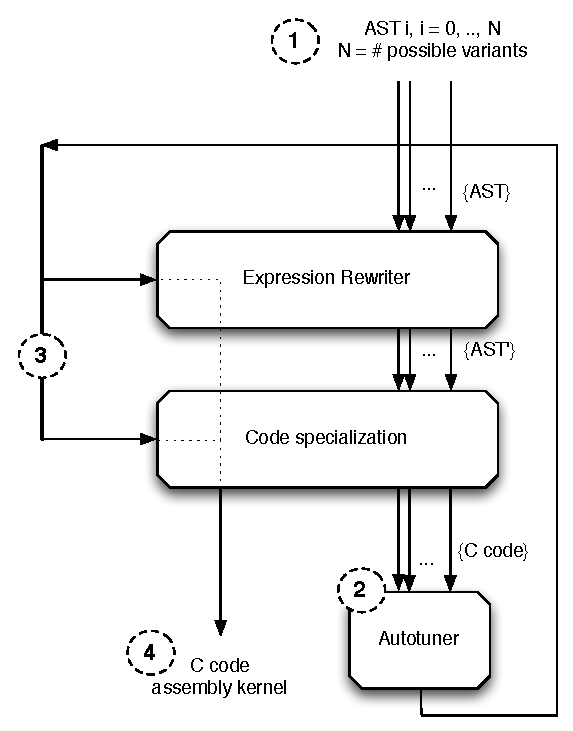
\includegraphics[scale=1.0]{pictures/coffee-scheme}
\label{fig:newcoffee}\caption{Overview of COFFEE. Numbers 1-2-3-4 indicate the flow.}
\end{center}
\end{figure}

\begin{figure}
\label{original-code}\caption{Original code}
\scriptsize
\lstinputlisting{listings/original.code}
\end{figure}

\begin{figure}
\label{zeros-code}\caption{Code after expression re-writing. Operations involving zero-valued entries in the arrays are removed by suitably adjusting the iteration space.}
\scriptsize
\lstinputlisting{listings/zeros.code}
\end{figure}

\begin{figure}
\label{zeros-tmps-code}\caption{Code after expression re-writing plus using temporaries to ensure aligned accesses.}
\scriptsize
\lstinputlisting{listings/zeros-tmps.code}
\end{figure}

Therefore, a possible thing to do for specializing code in a certain problem is
\begin{itemize}
\item Autotuning, based on domain-knowledge to keep the exploration space small enough
\end{itemize}
which would replace the cost model introduced in the COFFEE paper (here, we have more code variants). A scheme of the new COFFEE is in Figure~\ref{fig:newcoffee}
\end{itemize}


%We will have to prove  in significant applications showing also the speedup in the overall computation.

%\begin{thebibliography}{99}
%\setlength{\parskip}{0pt}
%
%\bibitem{FFC-Compiler} Robert~C. Kirby and Anders Logg. 
%\newblock A compiler for variational forms.
%\newblock {\em ACM Trans. Math. Softw.}, 32(3):417--444, September 2006.
%
%\end{thebibliography}

\end{document}